\section{Objectif du projet}

Le but du projet étant  tout d’abord de permettre aux étudiants d’allier théorie et pratique, nous allons reprendre ci-dessous les objectifs visés par ce projet.
Tout d’abord,  l’objectif premier étant de concevoir un amplificateur. Ce dernier  devant être muni d’un système de réglage de volume ainsi que des graves et aigus. Le signal étant envoyé à l’amplificateur depuis un smartphone ou un MP3.  De plus, la mise en pratique des concepts théoriques abordés tout au long du quadrimestre.
Le travail en groupe étant nécessaire lorsque l’on travaille sur un projet, nous avons dû apprendre  à faire des recherches  de manière plus ciblée ainsi qu’à nous organiser pour terminer nos travaux dans les temps.

\begin{figure}	
\begin{center}
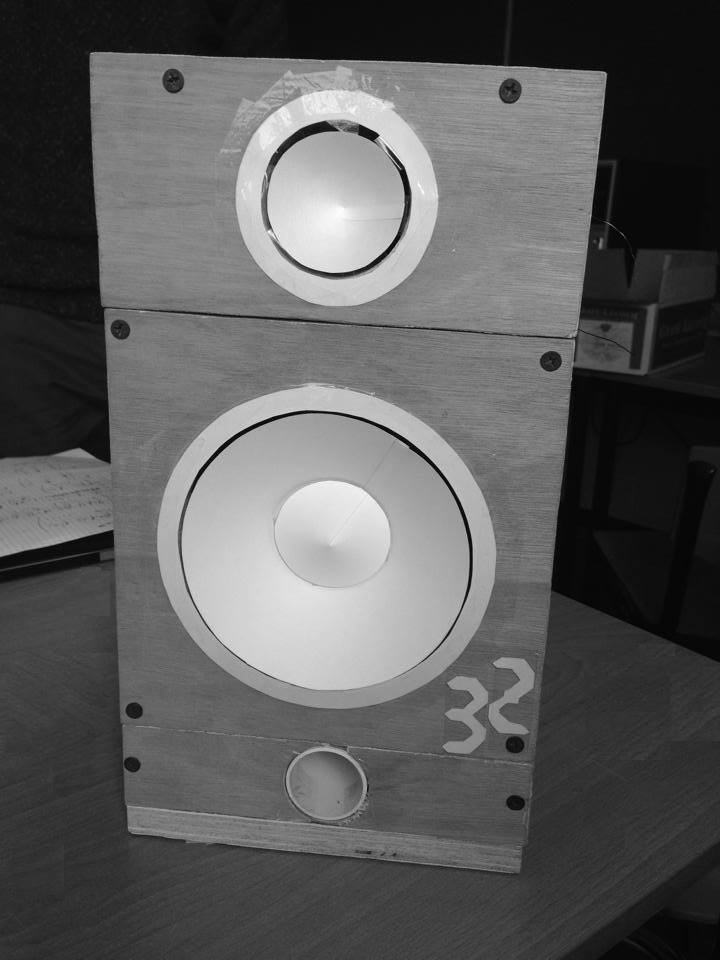
\includegraphics[scale=0.5]{img/PhotoHP} 
\end{center}
\caption{Rendu final des Hauts-Parleurs}		
\label{fig:PhotoHP}		
\end{figure}